\documentclass[1p]{elsarticle_modified}
%\bibliographystyle{elsarticle-num}

%\usepackage[colorlinks]{hyperref}
%\usepackage{abbrmath_seonhwa} %\Abb, \Ascr, \Acal ,\Abf, \Afrak
\usepackage{amsfonts}
\usepackage{amssymb}
\usepackage{amsmath}
\usepackage{amsthm}
\usepackage{scalefnt}
\usepackage{amsbsy}
\usepackage{kotex}
\usepackage{caption}
\usepackage{subfig}
\usepackage{color}
\usepackage{graphicx}
\usepackage{xcolor} %% white, black, red, green, blue, cyan, magenta, yellow
\usepackage{float}
\usepackage{setspace}
\usepackage{hyperref}

\usepackage{tikz}
\usetikzlibrary{arrows}

\usepackage{multirow}
\usepackage{array} % fixed length table
\usepackage{hhline}

%%%%%%%%%%%%%%%%%%%%%
\makeatletter
\renewcommand*\env@matrix[1][\arraystretch]{%
	\edef\arraystretch{#1}%
	\hskip -\arraycolsep
	\let\@ifnextchar\new@ifnextchar
	\array{*\c@MaxMatrixCols c}}
\makeatother %https://tex.stackexchange.com/questions/14071/how-can-i-increase-the-line-spacing-in-a-matrix
%%%%%%%%%%%%%%%

\usepackage[normalem]{ulem}

\newcommand{\msout}[1]{\ifmmode\text{\sout{\ensuremath{#1}}}\else\sout{#1}\fi}
%SOURCE: \msout is \stkout macro in https://tex.stackexchange.com/questions/20609/strikeout-in-math-mode

\newcommand{\cancel}[1]{
	\ifmmode
	{\color{red}\msout{#1}}
	\else
	{\color{red}\sout{#1}}
	\fi
}

\newcommand{\add}[1]{
	{\color{blue}\uwave{#1}}
}

\newcommand{\replace}[2]{
	\ifmmode
	{\color{red}\msout{#1}}{\color{blue}\uwave{#2}}
	\else
	{\color{red}\sout{#1}}{\color{blue}\uwave{#2}}
	\fi
}

\newcommand{\Sol}{\mathcal{S}} %segment
\newcommand{\D}{D} %diagram
\newcommand{\A}{\mathcal{A}} %arc


%%%%%%%%%%%%%%%%%%%%%%%%%%%%%5 test

\def\sl{\operatorname{\textup{SL}}(2,\Cbb)}
\def\psl{\operatorname{\textup{PSL}}(2,\Cbb)}
\def\quan{\mkern 1mu \triangleright \mkern 1mu}

\theoremstyle{definition}
\newtheorem{thm}{Theorem}[section]
\newtheorem{prop}[thm]{Proposition}
\newtheorem{lem}[thm]{Lemma}
\newtheorem{ques}[thm]{Question}
\newtheorem{cor}[thm]{Corollary}
\newtheorem{defn}[thm]{Definition}
\newtheorem{exam}[thm]{Example}
\newtheorem{rmk}[thm]{Remark}
\newtheorem{alg}[thm]{Algorithm}

\newcommand{\I}{\sqrt{-1}}
\begin{document}

%\begin{frontmatter}
%
%\title{Boundary parabolic representations of knots up to 8 crossings}
%
%%% Group authors per affiliation:
%\author{Yunhi Cho} 
%\address{Department of Mathematics, University of Seoul, Seoul, Korea}
%\ead{yhcho@uos.ac.kr}
%
%
%\author{Seonhwa Kim} %\fnref{s_kim}}
%\address{Center for Geometry and Physics, Institute for Basic Science, Pohang, 37673, Korea}
%\ead{ryeona17@ibs.re.kr}
%
%\author{Hyuk Kim}
%\address{Department of Mathematical Sciences, Seoul National University, Seoul 08826, Korea}
%\ead{hyukkim@snu.ac.kr}
%
%\author{Seokbeom Yoon}
%\address{Department of Mathematical Sciences, Seoul National University, Seoul, 08826,  Korea}
%\ead{sbyoon15@snu.ac.kr}
%
%\begin{abstract}
%We find all boundary parabolic representation of knots up to 8 crossings.
%
%\end{abstract}
%\begin{keyword}
%    \MSC[2010] 57M25 
%\end{keyword}
%
%\end{frontmatter}

%\linenumbers
%\tableofcontents
%
\newcommand\colored[1]{\textcolor{white}{\rule[-0.35ex]{0.8em}{1.4ex}}\kern-0.8em\color{red} #1}%
%\newcommand\colored[1]{\textcolor{white}{ #1}\kern-2.17ex	\textcolor{white}{ #1}\kern-1.81ex	\textcolor{white}{ #1}\kern-2.15ex\color{red}#1	}

{\Large $\underline{12a_{0741}~(K12a_{0741})}$}

\setlength{\tabcolsep}{10pt}
\renewcommand{\arraystretch}{1.6}
\vspace{1cm}\begin{tabular}{m{100pt}>{\centering\arraybackslash}m{274pt}}
\multirow{5}{120pt}{
	\centering
	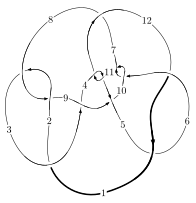
\includegraphics[width=112pt]{../../../GIT/diagram.site/Diagrams/png/1542_12a_0741.png}\\
\ \ \ A knot diagram\footnotemark}&
\allowdisplaybreaks
\textbf{Linearized knot diagam} \\
\cline{2-2}
 &
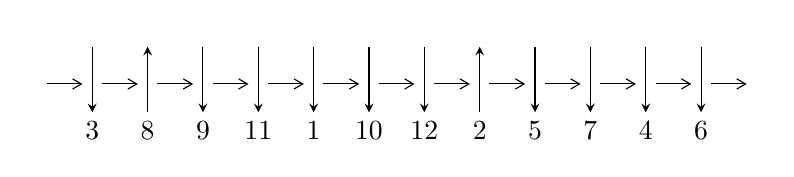
\begin{tikzpicture}[x=20pt, y=17pt]
	% nodes
	\node (C0) at (0, 0) {};
	\node (C1) at (1, 0) {};
	\node (C1U) at (1, +1) {};
	\node (C1D) at (1, -1) {3};

	\node (C2) at (2, 0) {};
	\node (C2U) at (2, +1) {};
	\node (C2D) at (2, -1) {8};

	\node (C3) at (3, 0) {};
	\node (C3U) at (3, +1) {};
	\node (C3D) at (3, -1) {9};

	\node (C4) at (4, 0) {};
	\node (C4U) at (4, +1) {};
	\node (C4D) at (4, -1) {11};

	\node (C5) at (5, 0) {};
	\node (C5U) at (5, +1) {};
	\node (C5D) at (5, -1) {1};

	\node (C6) at (6, 0) {};
	\node (C6U) at (6, +1) {};
	\node (C6D) at (6, -1) {10};

	\node (C7) at (7, 0) {};
	\node (C7U) at (7, +1) {};
	\node (C7D) at (7, -1) {12};

	\node (C8) at (8, 0) {};
	\node (C8U) at (8, +1) {};
	\node (C8D) at (8, -1) {2};

	\node (C9) at (9, 0) {};
	\node (C9U) at (9, +1) {};
	\node (C9D) at (9, -1) {5};

	\node (C10) at (10, 0) {};
	\node (C10U) at (10, +1) {};
	\node (C10D) at (10, -1) {7};

	\node (C11) at (11, 0) {};
	\node (C11U) at (11, +1) {};
	\node (C11D) at (11, -1) {4};

	\node (C12) at (12, 0) {};
	\node (C12U) at (12, +1) {};
	\node (C12D) at (12, -1) {6};
	\node (C13) at (13, 0) {};

	% arrows
	\draw[->,>={angle 60}]
	(C0) edge (C1) (C1) edge (C2) (C2) edge (C3) (C3) edge (C4) (C4) edge (C5) (C5) edge (C6) (C6) edge (C7) (C7) edge (C8) (C8) edge (C9) (C9) edge (C10) (C10) edge (C11) (C11) edge (C12) (C12) edge (C13) ;	\draw[->,>=stealth]
	(C1U) edge (C1D) (C2D) edge (C2U) (C3U) edge (C3D) (C4U) edge (C4D) (C5U) edge (C5D) (C6U) edge (C6D) (C7U) edge (C7D) (C8D) edge (C8U) (C9U) edge (C9D) (C10U) edge (C10D) (C11U) edge (C11D) (C12U) edge (C12D) ;
	\end{tikzpicture} \\
\hhline{~~} \\& 
\textbf{Solving Sequence} \\ \cline{2-2} 
 &
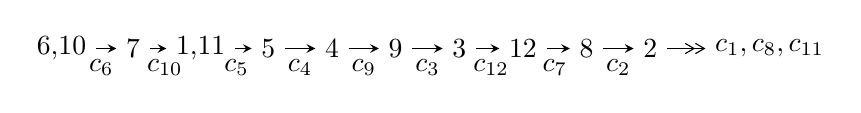
\begin{tikzpicture}[x=23pt, y=7pt]
	% node
	\node (A0) at (-1/8, 0) {6,10};
	\node (A1) at (1, 0) {7};
	\node (A2) at (33/16, 0) {1,11};
	\node (A3) at (25/8, 0) {5};
	\node (A4) at (33/8, 0) {4};
	\node (A5) at (41/8, 0) {9};
	\node (A6) at (49/8, 0) {3};
	\node (A7) at (57/8, 0) {12};
	\node (A8) at (65/8, 0) {8};
	\node (A9) at (73/8, 0) {2};
	\node (C1) at (1/2, -1) {$c_{6}$};
	\node (C2) at (3/2, -1) {$c_{10}$};
	\node (C3) at (21/8, -1) {$c_{5}$};
	\node (C4) at (29/8, -1) {$c_{4}$};
	\node (C5) at (37/8, -1) {$c_{9}$};
	\node (C6) at (45/8, -1) {$c_{3}$};
	\node (C7) at (53/8, -1) {$c_{12}$};
	\node (C8) at (61/8, -1) {$c_{7}$};
	\node (C9) at (69/8, -1) {$c_{2}$};
	\node (A10) at (11, 0) {$c_{1},c_{8},c_{11}$};

	% edge
	\draw[->,>=stealth]	
	(A0) edge (A1) (A1) edge (A2) (A2) edge (A3) (A3) edge (A4) (A4) edge (A5) (A5) edge (A6) (A6) edge (A7) (A7) edge (A8) (A8) edge (A9) ;
	\draw[->>,>={angle 60}]	
	(A9) edge (A10);
\end{tikzpicture} \\ 

\end{tabular} \\

\footnotetext{
The image of knot diagram is generated by the software ``\textbf{Draw programme}" developed by Andrew Bartholomew(\url{http://www.layer8.co.uk/maths/draw/index.htm\#Running-draw}), where we modified some parts for our purpose(\url{https://github.com/CATsTAILs/LinksPainter}).
}\phantom \\ \newline 
\centering \textbf{Ideals for irreducible components\footnotemark of $X_{\text{par}}$} 
 
\begin{align*}
I^u_{1}&=\langle 
-9.22629\times10^{114} u^{52}-2.74007\times10^{115} u^{51}+\cdots+4.77254\times10^{116} b+2.56825\times10^{117},\\
\phantom{I^u_{1}}&\phantom{= \langle  }1.04478\times10^{116} u^{52}+3.89252\times10^{116} u^{51}+\cdots+1.90902\times10^{118} a-3.41478\times10^{118},\\
\phantom{I^u_{1}}&\phantom{= \langle  }u^{53}+2 u^{52}+\cdots+329 u+160\rangle \\
I^u_{2}&=\langle 
u^{38}+u^{37}+\cdots+a+2,\;2 u^{38} a+14 u^{38}+\cdots+6 a+14,\;u^{39}+u^{38}+\cdots+2 u+1\rangle \\
I^u_{3}&=\langle 
b-1,\;16 a^4-32 a^3+16 a^2+1,\;u+1\rangle \\
I^u_{4}&=\langle 
-4 u^2 a+a u-13 u^2+23 b+10 a+9 u-25,\;-70 u^2 a+25 a^2+40 a u+151 u^2-130 a-62 u+309,\\
\phantom{I^u_{4}}&\phantom{= \langle  }u^3- u^2+2 u-1\rangle \\
I^u_{5}&=\langle 
b+1,\;8 a^3+12 a^2+6 a+1,\;u-1\rangle \\
\\
\end{align*}
\raggedright * 5 irreducible components of $\dim_{\mathbb{C}}=0$, with total 144 representations.\\
\footnotetext{All coefficients of polynomials are rational numbers. But the coefficients are sometimes approximated in decimal forms when there is not enough margin.}
\newpage
\renewcommand{\arraystretch}{1}
\centering \section*{I. $I^u_{1}= \langle -9.23\times10^{114} u^{52}-2.74\times10^{115} u^{51}+\cdots+4.77\times10^{116} b+2.57\times10^{117},\;1.04\times10^{116} u^{52}+3.89\times10^{116} u^{51}+\cdots+1.91\times10^{118} a-3.41\times10^{118},\;u^{53}+2 u^{52}+\cdots+329 u+160 \rangle$}
\flushleft \textbf{(i) Arc colorings}\\
\begin{tabular}{m{7pt} m{180pt} m{7pt} m{180pt} }
\flushright $a_{6}=$&$\begin{pmatrix}1\\0\end{pmatrix}$ \\
\flushright $a_{10}=$&$\begin{pmatrix}0\\u\end{pmatrix}$ \\
\flushright $a_{7}=$&$\begin{pmatrix}1\\u^2\end{pmatrix}$ \\
\flushright $a_{1}=$&$\begin{pmatrix}-0.00547287 u^{52}-0.0203902 u^{51}+\cdots-5.89017 u+1.78876\\0.0193320 u^{52}+0.0574133 u^{51}+\cdots-12.8760 u-5.38131\end{pmatrix}$ \\
\flushright $a_{11}=$&$\begin{pmatrix}- u\\- u^3+u\end{pmatrix}$ \\
\flushright $a_{5}=$&$\begin{pmatrix}0.0243283 u^{52}+0.0637946 u^{51}+\cdots-4.49363 u+0.406738\\0.0256578 u^{52}+0.0667823 u^{51}+\cdots-17.0251 u-4.63953\end{pmatrix}$ \\
\flushright $a_{4}=$&$\begin{pmatrix}0.0430776 u^{52}+0.111948 u^{51}+\cdots-16.2352 u-2.68638\\0.0138491 u^{52}+0.0344025 u^{51}+\cdots-11.7889 u-3.25117\end{pmatrix}$ \\
\flushright $a_{9}=$&$\begin{pmatrix}0.0196369 u^{52}+0.0612628 u^{51}+\cdots-3.78192 u-4.37932\\-0.00126582 u^{52}-0.00958516 u^{51}+\cdots-0.909111 u+0.348371\end{pmatrix}$ \\
\flushright $a_{3}=$&$\begin{pmatrix}0.0151668 u^{52}+0.0328572 u^{51}+\cdots-12.7531 u-1.36568\\-0.0100144 u^{52}-0.0235824 u^{51}+\cdots+0.705795 u-0.528707\end{pmatrix}$ \\
\flushright $a_{12}=$&$\begin{pmatrix}0.0138591 u^{52}+0.0370231 u^{51}+\cdots-18.7662 u-3.59254\\0.0193320 u^{52}+0.0574133 u^{51}+\cdots-12.8760 u-5.38131\end{pmatrix}$ \\
\flushright $a_{8}=$&$\begin{pmatrix}-0.0241663 u^{52}-0.0663621 u^{51}+\cdots+3.16247 u+1.51646\\0.00213415 u^{52}+0.00509088 u^{51}+\cdots-1.04158 u-0.257202\end{pmatrix}$ \\
\flushright $a_{2}=$&$\begin{pmatrix}0.00119343 u^{52}-0.0121666 u^{51}+\cdots-6.31916 u+1.10586\\-0.0242121 u^{52}-0.0727143 u^{51}+\cdots+5.31037 u+2.13761\end{pmatrix}$\\&\end{tabular}
\flushleft \textbf{(ii) Obstruction class $= -1$}\\~\\
\flushleft \textbf{(iii) Cusp Shapes $= 0.102716 u^{52}+0.362833 u^{51}+\cdots+2.34272 u-23.6794$}\\~\\
\newpage\renewcommand{\arraystretch}{1}
\flushleft \textbf{(iv) u-Polynomials at the component}\newline \\
\begin{tabular}{m{50pt}|m{274pt}}
Crossings & \hspace{64pt}u-Polynomials at each crossing \\
\hline $$\begin{aligned}c_{1}\end{aligned}$$&$\begin{aligned}
&u^{53}+25 u^{52}+\cdots-112 u-64
\end{aligned}$\\
\hline $$\begin{aligned}c_{2},c_{8}\end{aligned}$$&$\begin{aligned}
&u^{53}-3 u^{52}+\cdots-12 u+8
\end{aligned}$\\
\hline $$\begin{aligned}c_{3}\end{aligned}$$&$\begin{aligned}
&u^{53}+3 u^{52}+\cdots+91812 u+11464
\end{aligned}$\\
\hline $$\begin{aligned}c_{4},c_{5},c_{11}\\c_{12}\end{aligned}$$&$\begin{aligned}
&u^{53}- u^{52}+\cdots-2 u+1
\end{aligned}$\\
\hline $$\begin{aligned}c_{6},c_{10}\end{aligned}$$&$\begin{aligned}
&u^{53}+2 u^{52}+\cdots+329 u+160
\end{aligned}$\\
\hline $$\begin{aligned}c_{7},c_{9}\end{aligned}$$&$\begin{aligned}
&128(128 u^{53}-64 u^{52}+\cdots-13 u+1)
\end{aligned}$\\
\hline
\end{tabular}\\~\\
\newpage\renewcommand{\arraystretch}{1}
\flushleft \textbf{(v) Riley Polynomials at the component}\newline \\
\begin{tabular}{m{50pt}|m{274pt}}
Crossings & \hspace{64pt}Riley Polynomials at each crossing \\
\hline $$\begin{aligned}c_{1}\end{aligned}$$&$\begin{aligned}
&y^{53}+9 y^{52}+\cdots-3840 y-4096
\end{aligned}$\\
\hline $$\begin{aligned}c_{2},c_{8}\end{aligned}$$&$\begin{aligned}
&y^{53}+25 y^{52}+\cdots-112 y-64
\end{aligned}$\\
\hline $$\begin{aligned}c_{3}\end{aligned}$$&$\begin{aligned}
&y^{53}-7 y^{52}+\cdots+828536208 y-131423296
\end{aligned}$\\
\hline $$\begin{aligned}c_{4},c_{5},c_{11}\\c_{12}\end{aligned}$$&$\begin{aligned}
&y^{53}+17 y^{52}+\cdots-18 y-1
\end{aligned}$\\
\hline $$\begin{aligned}c_{6},c_{10}\end{aligned}$$&$\begin{aligned}
&y^{53}-22 y^{52}+\cdots+992401 y-25600
\end{aligned}$\\
\hline $$\begin{aligned}c_{7},c_{9}\end{aligned}$$&$\begin{aligned}
&16384(16384 y^{53}-208896 y^{52}+\cdots-135 y-1)
\end{aligned}$\\
\hline
\end{tabular}\\~\\
\newpage\flushleft \textbf{(vi) Complex Volumes and Cusp Shapes}
$$\begin{array}{c|c|c}  
\text{Solutions to }I^u_{1}& \I (\text{vol} + \sqrt{-1}CS) & \text{Cusp shape}\\
 \hline 
\begin{aligned}
u &= \phantom{-}1.010500 + 0.277494 I \\
a &= -0.309112 + 0.248738 I \\
b &= -1.230130 + 0.452325 I\end{aligned}
 & -3.60132 - 1.23088 I & -8.16326 + 5.88240 I \\ \hline\begin{aligned}
u &= \phantom{-}1.010500 - 0.277494 I \\
a &= -0.309112 - 0.248738 I \\
b &= -1.230130 - 0.452325 I\end{aligned}
 & -3.60132 + 1.23088 I & -8.16326 - 5.88240 I \\ \hline\begin{aligned}
u &= -1.016340 + 0.336995 I \\
a &= \phantom{-}0.237630 + 0.305698 I \\
b &= \phantom{-}1.31165 + 0.53324 I\end{aligned}
 & -5.96983 + 5.72038 I & -11.2924 - 8.5433 I \\ \hline\begin{aligned}
u &= -1.016340 - 0.336995 I \\
a &= \phantom{-}0.237630 - 0.305698 I \\
b &= \phantom{-}1.31165 - 0.53324 I\end{aligned}
 & -5.96983 - 5.72038 I & -11.2924 + 8.5433 I \\ \hline\begin{aligned}
u &= \phantom{-}0.894368 + 0.170124 I \\
a &= -1.173990 + 0.551696 I \\
b &= \phantom{-}0.192195 - 0.262622 I\end{aligned}
 & -4.05202 + 3.78789 I & -10.53464 - 4.24172 I \\ \hline\begin{aligned}
u &= \phantom{-}0.894368 - 0.170124 I \\
a &= -1.173990 - 0.551696 I \\
b &= \phantom{-}0.192195 + 0.262622 I\end{aligned}
 & -4.05202 - 3.78789 I & -10.53464 + 4.24172 I \\ \hline\begin{aligned}
u &= \phantom{-}0.889815 + 0.158884 I \\
a &= -0.558076 + 0.216460 I \\
b &= -1.237620 + 0.182509 I\end{aligned}
 & -2.84156 - 0.53577 I & -2.03217 + 7.98267 I \\ \hline\begin{aligned}
u &= \phantom{-}0.889815 - 0.158884 I \\
a &= -0.558076 - 0.216460 I \\
b &= -1.237620 - 0.182509 I\end{aligned}
 & -2.84156 + 0.53577 I & -2.03217 - 7.98267 I \\ \hline\begin{aligned}
u &= \phantom{-}0.856411 + 0.685171 I \\
a &= \phantom{-}0.23931 - 1.74388 I \\
b &= \phantom{-}0.468215 + 0.785484 I\end{aligned}
 & -4.04273 + 0.39813 I & -11.01909 + 4.12127 I \\ \hline\begin{aligned}
u &= \phantom{-}0.856411 - 0.685171 I \\
a &= \phantom{-}0.23931 + 1.74388 I \\
b &= \phantom{-}0.468215 - 0.785484 I\end{aligned}
 & -4.04273 - 0.39813 I & -11.01909 - 4.12127 I\\
 \hline 
 \end{array}$$\newpage$$\begin{array}{c|c|c}  
\text{Solutions to }I^u_{1}& \I (\text{vol} + \sqrt{-1}CS) & \text{Cusp shape}\\
 \hline 
\begin{aligned}
u &= -0.357016 + 1.088740 I \\
a &= \phantom{-}0.29731 + 1.45796 I \\
b &= -0.487890 - 1.101780 I\end{aligned}
 & \phantom{-}0.44124 - 4.68393 I & -8.30547 + 4.38111 I \\ \hline\begin{aligned}
u &= -0.357016 - 1.088740 I \\
a &= \phantom{-}0.29731 - 1.45796 I \\
b &= -0.487890 + 1.101780 I\end{aligned}
 & \phantom{-}0.44124 + 4.68393 I & -8.30547 - 4.38111 I \\ \hline\begin{aligned}
u &= -1.107520 + 0.302023 I \\
a &= \phantom{-}0.185994 + 0.166983 I \\
b &= \phantom{-}1.135680 + 0.628747 I\end{aligned}
 & -7.15683 - 1.71285 I & -15.0160 - 0.3603 I \\ \hline\begin{aligned}
u &= -1.107520 - 0.302023 I \\
a &= \phantom{-}0.185994 - 0.166983 I \\
b &= \phantom{-}1.135680 - 0.628747 I\end{aligned}
 & -7.15683 + 1.71285 I & -15.0160 + 0.3603 I \\ \hline\begin{aligned}
u &= -0.246858 + 1.143050 I \\
a &= \phantom{-}0.22408 + 1.48798 I \\
b &= -0.507181 - 1.240200 I\end{aligned}
 & \phantom{-}3.35515 - 13.11250 I & -5.16195 + 8.65922 I \\ \hline\begin{aligned}
u &= -0.246858 - 1.143050 I \\
a &= \phantom{-}0.22408 - 1.48798 I \\
b &= -0.507181 + 1.240200 I\end{aligned}
 & \phantom{-}3.35515 + 13.11250 I & -5.16195 - 8.65922 I \\ \hline\begin{aligned}
u &= \phantom{-}0.285314 + 1.165920 I \\
a &= -0.23055 + 1.46085 I \\
b &= \phantom{-}0.460429 - 1.210720 I\end{aligned}
 & \phantom{-}5.76708 + 7.70183 I & -2.26158 - 5.23055 I \\ \hline\begin{aligned}
u &= \phantom{-}0.285314 - 1.165920 I \\
a &= -0.23055 - 1.46085 I \\
b &= \phantom{-}0.460429 + 1.210720 I\end{aligned}
 & \phantom{-}5.76708 - 7.70183 I & -2.26158 + 5.23055 I \\ \hline\begin{aligned}
u &= -1.190920 + 0.164534 I \\
a &= \phantom{-}0.595741 + 0.422528 I \\
b &= \phantom{-}0.162888 - 0.445268 I\end{aligned}
 & -1.54684 + 0.49363 I & -7.46237 - 2.14913 I \\ \hline\begin{aligned}
u &= -1.190920 - 0.164534 I \\
a &= \phantom{-}0.595741 - 0.422528 I \\
b &= \phantom{-}0.162888 + 0.445268 I\end{aligned}
 & -1.54684 - 0.49363 I & -7.46237 + 2.14913 I\\
 \hline 
 \end{array}$$\newpage$$\begin{array}{c|c|c}  
\text{Solutions to }I^u_{1}& \I (\text{vol} + \sqrt{-1}CS) & \text{Cusp shape}\\
 \hline 
\begin{aligned}
u &= -0.957980 + 0.787698 I \\
a &= -0.37852 - 1.57550 I \\
b &= -0.434771 + 0.898967 I\end{aligned}
 & -0.60629 + 4.29298 I & -8.00000 - 7.47231 I \\ \hline\begin{aligned}
u &= -0.957980 - 0.787698 I \\
a &= -0.37852 + 1.57550 I \\
b &= -0.434771 - 0.898967 I\end{aligned}
 & -0.60629 - 4.29298 I & -8.00000 + 7.47231 I \\ \hline\begin{aligned}
u &= \phantom{-}1.041380 + 0.692963 I \\
a &= \phantom{-}0.56731 - 1.66360 I \\
b &= \phantom{-}0.542920 + 0.942914 I\end{aligned}
 & -4.64111 - 8.53246 I & -11.2112 + 9.6162 I \\ \hline\begin{aligned}
u &= \phantom{-}1.041380 - 0.692963 I \\
a &= \phantom{-}0.56731 + 1.66360 I \\
b &= \phantom{-}0.542920 - 0.942914 I\end{aligned}
 & -4.64111 + 8.53246 I & -11.2112 - 9.6162 I \\ \hline\begin{aligned}
u &= -0.738902 + 0.118991 I \\
a &= \phantom{-}0.839648 + 0.253541 I \\
b &= \phantom{-}1.328440 + 0.061804 I\end{aligned}
 & -4.61573 - 3.33353 I & -5.28986 + 1.76068 I \\ \hline\begin{aligned}
u &= -0.738902 - 0.118991 I \\
a &= \phantom{-}0.839648 - 0.253541 I \\
b &= \phantom{-}1.328440 - 0.061804 I\end{aligned}
 & -4.61573 + 3.33353 I & -5.28986 - 1.76068 I \\ \hline\begin{aligned}
u &= \phantom{-}1.309210 + 0.191706 I \\
a &= -0.150987 - 0.150085 I \\
b &= -0.689475 + 0.753211 I\end{aligned}
 & -5.84739 + 0.86218 I & \phantom{-0.000000 } 0 \\ \hline\begin{aligned}
u &= \phantom{-}1.309210 - 0.191706 I \\
a &= -0.150987 + 0.150085 I \\
b &= -0.689475 - 0.753211 I\end{aligned}
 & -5.84739 - 0.86218 I & \phantom{-0.000000 } 0 \\ \hline\begin{aligned}
u &= \phantom{-}0.455502 + 1.311390 I \\
a &= -0.229330 + 1.339160 I \\
b &= \phantom{-}0.293604 - 1.116830 I\end{aligned}
 & \phantom{-}7.73147 + 4.14673 I & \phantom{-0.000000 } 0 \\ \hline\begin{aligned}
u &= \phantom{-}0.455502 - 1.311390 I \\
a &= -0.229330 - 1.339160 I \\
b &= \phantom{-}0.293604 + 1.116830 I\end{aligned}
 & \phantom{-}7.73147 - 4.14673 I & \phantom{-0.000000 } 0\\
 \hline 
 \end{array}$$\newpage$$\begin{array}{c|c|c}  
\text{Solutions to }I^u_{1}& \I (\text{vol} + \sqrt{-1}CS) & \text{Cusp shape}\\
 \hline 
\begin{aligned}
u &= -1.253370 + 0.652070 I \\
a &= -0.94701 - 1.36034 I \\
b &= -0.633605 + 1.227090 I\end{aligned}
 & -2.43644 + 10.92000 I & \phantom{-0.000000 } 0 \\ \hline\begin{aligned}
u &= -1.253370 - 0.652070 I \\
a &= -0.94701 + 1.36034 I \\
b &= -0.633605 - 1.227090 I\end{aligned}
 & -2.43644 - 10.92000 I & \phantom{-0.000000 } 0 \\ \hline\begin{aligned}
u &= -1.29214 + 0.64007 I \\
a &= -1.01211 - 1.27074 I \\
b &= -0.64920 + 1.30689 I\end{aligned}
 & \phantom{-}0.0577 + 19.4085 I & \phantom{-0.000000 } 0 \\ \hline\begin{aligned}
u &= -1.29214 - 0.64007 I \\
a &= -1.01211 + 1.27074 I \\
b &= -0.64920 - 1.30689 I\end{aligned}
 & \phantom{-}0.0577 - 19.4085 I & \phantom{-0.000000 } 0 \\ \hline\begin{aligned}
u &= \phantom{-}1.28693 + 0.65572 I \\
a &= \phantom{-}0.96664 - 1.27292 I \\
b &= \phantom{-}0.61846 + 1.29081 I\end{aligned}
 & \phantom{-}2.5806 - 14.1172 I & \phantom{-0.000000 } 0 \\ \hline\begin{aligned}
u &= \phantom{-}1.28693 - 0.65572 I \\
a &= \phantom{-}0.96664 + 1.27292 I \\
b &= \phantom{-}0.61846 - 1.29081 I\end{aligned}
 & \phantom{-}2.5806 + 14.1172 I & \phantom{-0.000000 } 0 \\ \hline\begin{aligned}
u &= \phantom{-}1.28431 + 0.72559 I \\
a &= \phantom{-}0.80342 - 1.23877 I \\
b &= \phantom{-}0.498243 + 1.251700 I\end{aligned}
 & \phantom{-}4.89820 - 11.20600 I & \phantom{-0.000000 } 0 \\ \hline\begin{aligned}
u &= \phantom{-}1.28431 - 0.72559 I \\
a &= \phantom{-}0.80342 + 1.23877 I \\
b &= \phantom{-}0.498243 - 1.251700 I\end{aligned}
 & \phantom{-}4.89820 + 11.20600 I & \phantom{-0.000000 } 0 \\ \hline\begin{aligned}
u &= -1.27009 + 0.77458 I \\
a &= -0.70606 - 1.24445 I \\
b &= -0.441345 + 1.205700 I\end{aligned}
 & \phantom{-}4.39290 + 5.76841 I & \phantom{-0.000000 } 0 \\ \hline\begin{aligned}
u &= -1.27009 - 0.77458 I \\
a &= -0.70606 + 1.24445 I \\
b &= -0.441345 - 1.205700 I\end{aligned}
 & \phantom{-}4.39290 - 5.76841 I & \phantom{-0.000000 } 0\\
 \hline 
 \end{array}$$\newpage$$\begin{array}{c|c|c}  
\text{Solutions to }I^u_{1}& \I (\text{vol} + \sqrt{-1}CS) & \text{Cusp shape}\\
 \hline 
\begin{aligned}
u &= -0.62038 + 1.36139 I \\
a &= \phantom{-}0.247137 + 1.266590 I \\
b &= -0.239949 - 1.046860 I\end{aligned}
 & \phantom{-}6.83679 + 1.68050 I & \phantom{-0.000000 } 0 \\ \hline\begin{aligned}
u &= -0.62038 - 1.36139 I \\
a &= \phantom{-}0.247137 - 1.266590 I \\
b &= -0.239949 + 1.046860 I\end{aligned}
 & \phantom{-}6.83679 - 1.68050 I & \phantom{-0.000000 } 0 \\ \hline\begin{aligned}
u &= -1.50653 + 0.08391 I \\
a &= \phantom{-}0.136195 - 0.401648 I \\
b &= \phantom{-}0.397232 + 0.840006 I\end{aligned}
 & -1.12611 - 2.71991 I & \phantom{-0.000000 } 0 \\ \hline\begin{aligned}
u &= -1.50653 - 0.08391 I \\
a &= \phantom{-}0.136195 + 0.401648 I \\
b &= \phantom{-}0.397232 - 0.840006 I\end{aligned}
 & -1.12611 + 2.71991 I & \phantom{-0.000000 } 0 \\ \hline\begin{aligned}
u &= -0.18082 + 1.50804 I \\
a &= -0.025191 - 1.242950 I \\
b &= -0.035651 + 0.846395 I\end{aligned}
 & \phantom{-}5.62880 + 2.99985 I & \phantom{-0.000000 } 0 \\ \hline\begin{aligned}
u &= -0.18082 - 1.50804 I \\
a &= -0.025191 + 1.242950 I \\
b &= -0.035651 - 0.846395 I\end{aligned}
 & \phantom{-}5.62880 - 2.99985 I & \phantom{-0.000000 } 0 \\ \hline\begin{aligned}
u &= \phantom{-}1.52320 + 0.19708 I \\
a &= -0.031722 - 0.366987 I \\
b &= -0.453417 + 0.944633 I\end{aligned}
 & -3.01084 + 7.94270 I & \phantom{-0.000000 } 0 \\ \hline\begin{aligned}
u &= \phantom{-}1.52320 - 0.19708 I \\
a &= -0.031722 + 0.366987 I \\
b &= -0.453417 - 0.944633 I\end{aligned}
 & -3.01084 - 7.94270 I & \phantom{-0.000000 } 0 \\ \hline\begin{aligned}
u &= -0.279211 + 0.248748 I \\
a &= \phantom{-}0.598547 - 0.883823 I \\
b &= -0.239491 + 0.269538 I\end{aligned}
 & -0.533461 + 0.879212 I & -9.52326 - 7.63662 I \\ \hline\begin{aligned}
u &= -0.279211 - 0.248748 I \\
a &= \phantom{-}0.598547 + 0.883823 I \\
b &= -0.239491 - 0.269538 I\end{aligned}
 & -0.533461 - 0.879212 I & -9.52326 + 7.63662 I\\
 \hline 
 \end{array}$$\newpage$$\begin{array}{c|c|c}  
\text{Solutions to }I^u_{1}& \I (\text{vol} + \sqrt{-1}CS) & \text{Cusp shape}\\
 \hline 
\begin{aligned}
u &= \phantom{-}0.349659 + 0.074107 I \\
a &= -2.23401 + 1.00440 I \\
b &= \phantom{-}0.596328 - 0.151333 I\end{aligned}
 & -3.95805 + 3.86479 I & -11.90700 - 4.97851 I \\ \hline\begin{aligned}
u &= \phantom{-}0.349659 - 0.074107 I \\
a &= -2.23401 - 1.00440 I \\
b &= \phantom{-}0.596328 + 0.151333 I\end{aligned}
 & -3.95805 - 3.86479 I & -11.90700 + 4.97851 I \\ \hline\begin{aligned}
u &= -0.337034\phantom{ +0.000000I} \\
a &= \phantom{-}1.65164\phantom{ +0.000000I} \\
b &= -0.453134\phantom{ +0.000000I}\end{aligned}
 & -1.01554\phantom{ +0.000000I} & -10.2060\phantom{ +0.000000I}\\
 \hline 
 \end{array}$$\newpage\newpage\renewcommand{\arraystretch}{1}
\centering \section*{II. $I^u_{2}= \langle u^{38}+u^{37}+\cdots+a+2,\;2 u^{38} a+14 u^{38}+\cdots+6 a+14,\;u^{39}+u^{38}+\cdots+2 u+1 \rangle$}
\flushleft \textbf{(i) Arc colorings}\\
\begin{tabular}{m{7pt} m{180pt} m{7pt} m{180pt} }
\flushright $a_{6}=$&$\begin{pmatrix}1\\0\end{pmatrix}$ \\
\flushright $a_{10}=$&$\begin{pmatrix}0\\u\end{pmatrix}$ \\
\flushright $a_{7}=$&$\begin{pmatrix}1\\u^2\end{pmatrix}$ \\
\flushright $a_{1}=$&$\begin{pmatrix}a\\- u^{38}- u^{37}+\cdots- a-2\end{pmatrix}$ \\
\flushright $a_{11}=$&$\begin{pmatrix}- u\\- u^3+u\end{pmatrix}$ \\
\flushright $a_{5}=$&$\begin{pmatrix}- u^{38} a-4 u^{38}+\cdots-2 a-2\\u^5 a+u^6-2 u^3 a-2 u^4+a u+2 u^2\end{pmatrix}$ \\
\flushright $a_{4}=$&$\begin{pmatrix}- u^{38} a-4 u^{38}+\cdots-2 a-3\\1\end{pmatrix}$ \\
\flushright $a_{9}=$&$\begin{pmatrix}-2 u^{38} a-10 u^{38}+\cdots- a-10\\u^{38}- u^{37}+\cdots+a+4\end{pmatrix}$ \\
\flushright $a_{3}=$&$\begin{pmatrix}- u^{38} a-3 u^{37} a+\cdots+12 u+7\\-2 u^{38}-2 u^{37}+\cdots+a u+2 u\end{pmatrix}$ \\
\flushright $a_{12}=$&$\begin{pmatrix}- u^{38}- u^{37}+\cdots-2 u-2\\- u^{38}- u^{37}+\cdots- a-2\end{pmatrix}$ \\
\flushright $a_{8}=$&$\begin{pmatrix}u^{38} a+10 u^{38}+\cdots+4 a+13\\-2 u^{38}-2 u^{37}+\cdots+2 u-1\end{pmatrix}$ \\
\flushright $a_{2}=$&$\begin{pmatrix}- u^{38} a-11 u^{38}+\cdots+24 u+6\\u^{37} a- u^{38}+\cdots+a u+2 u\end{pmatrix}$\\&\end{tabular}
\flushleft \textbf{(ii) Obstruction class $= -1$}\\~\\
\flushleft \textbf{(iii) Cusp Shapes $= -4 u^{38}+44 u^{36}+4 u^{35}-232 u^{34}-40 u^{33}+752 u^{32}+192 u^{31}-1620 u^{30}-564 u^{29}+2316 u^{28}+1092 u^{27}-1948 u^{26}-1380 u^{25}+284 u^{24}+980 u^{23}+1508 u^{22}-16 u^{21}-1892 u^{20}-728 u^{19}+776 u^{18}+660 u^{17}+444 u^{16}-64 u^{15}-692 u^{14}-332 u^{13}+236 u^{12}+252 u^{11}+128 u^{10}+4 u^9-132 u^8-96 u^7+20 u^6+40 u^5+20 u^4+8 u^3-8 u^2-12 u-14$}\\~\\
\newpage\renewcommand{\arraystretch}{1}
\flushleft \textbf{(iv) u-Polynomials at the component}\newline \\
\begin{tabular}{m{50pt}|m{274pt}}
Crossings & \hspace{64pt}u-Polynomials at each crossing \\
\hline $$\begin{aligned}c_{1}\end{aligned}$$&$\begin{aligned}
&(u^{39}+19 u^{38}+\cdots+2 u^2-1)^{2}
\end{aligned}$\\
\hline $$\begin{aligned}c_{2},c_{8}\end{aligned}$$&$\begin{aligned}
&(u^{39}+u^{38}+\cdots+2 u^3-1)^{2}
\end{aligned}$\\
\hline $$\begin{aligned}c_{3}\end{aligned}$$&$\begin{aligned}
&(u^{39}- u^{38}+\cdots-18 u-17)^{2}
\end{aligned}$\\
\hline $$\begin{aligned}c_{4},c_{5},c_{11}\\c_{12}\end{aligned}$$&$\begin{aligned}
&u^{78}+3 u^{77}+\cdots+788 u+173
\end{aligned}$\\
\hline $$\begin{aligned}c_{6},c_{10}\end{aligned}$$&$\begin{aligned}
&(u^{39}+u^{38}+\cdots+2 u+1)^{2}
\end{aligned}$\\
\hline $$\begin{aligned}c_{7},c_{9}\end{aligned}$$&$\begin{aligned}
&u^{78}-21 u^{77}+\cdots+448674 u+57751
\end{aligned}$\\
\hline
\end{tabular}\\~\\
\newpage\renewcommand{\arraystretch}{1}
\flushleft \textbf{(v) Riley Polynomials at the component}\newline \\
\begin{tabular}{m{50pt}|m{274pt}}
Crossings & \hspace{64pt}Riley Polynomials at each crossing \\
\hline $$\begin{aligned}c_{1}\end{aligned}$$&$\begin{aligned}
&(y^{39}+3 y^{38}+\cdots+4 y-1)^{2}
\end{aligned}$\\
\hline $$\begin{aligned}c_{2},c_{8}\end{aligned}$$&$\begin{aligned}
&(y^{39}+19 y^{38}+\cdots+2 y^2-1)^{2}
\end{aligned}$\\
\hline $$\begin{aligned}c_{3}\end{aligned}$$&$\begin{aligned}
&(y^{39}-13 y^{38}+\cdots+3588 y-289)^{2}
\end{aligned}$\\
\hline $$\begin{aligned}c_{4},c_{5},c_{11}\\c_{12}\end{aligned}$$&$\begin{aligned}
&y^{78}+47 y^{77}+\cdots+318100 y+29929
\end{aligned}$\\
\hline $$\begin{aligned}c_{6},c_{10}\end{aligned}$$&$\begin{aligned}
&(y^{39}-21 y^{38}+\cdots+2 y^2-1)^{2}
\end{aligned}$\\
\hline $$\begin{aligned}c_{7},c_{9}\end{aligned}$$&$\begin{aligned}
&y^{78}+27 y^{77}+\cdots-879585708 y+3335178001
\end{aligned}$\\
\hline
\end{tabular}\\~\\
\newpage\flushleft \textbf{(vi) Complex Volumes and Cusp Shapes}
$$\begin{array}{c|c|c}  
\text{Solutions to }I^u_{2}& \I (\text{vol} + \sqrt{-1}CS) & \text{Cusp shape}\\
 \hline 
\begin{aligned}
u &= -0.913577 + 0.379498 I \\
a &= -1.64226 - 0.07520 I \\
b &= -0.477548 + 0.774232 I\end{aligned}
 & \phantom{-}1.22606 + 1.25772 I & -10.67108 - 2.89583 I \\ \hline\begin{aligned}
u &= -0.913577 + 0.379498 I \\
a &= \phantom{-}0.62112 + 1.52499 I \\
b &= -0.068253 - 1.290290 I\end{aligned}
 & \phantom{-}1.22606 + 1.25772 I & -10.67108 - 2.89583 I \\ \hline\begin{aligned}
u &= -0.913577 - 0.379498 I \\
a &= -1.64226 + 0.07520 I \\
b &= -0.477548 - 0.774232 I\end{aligned}
 & \phantom{-}1.22606 - 1.25772 I & -10.67108 + 2.89583 I \\ \hline\begin{aligned}
u &= -0.913577 - 0.379498 I \\
a &= \phantom{-}0.62112 - 1.52499 I \\
b &= -0.068253 + 1.290290 I\end{aligned}
 & \phantom{-}1.22606 - 1.25772 I & -10.67108 + 2.89583 I \\ \hline\begin{aligned}
u &= -0.867921 + 0.539600 I \\
a &= \phantom{-}0.510917 + 0.983764 I \\
b &= -0.18434 - 1.52434 I\end{aligned}
 & \phantom{-}3.26214 + 7.71489 I & -5.96279 - 8.94046 I \\ \hline\begin{aligned}
u &= -0.867921 + 0.539600 I \\
a &= -1.238810 - 0.665421 I \\
b &= -0.787918 + 1.001630 I\end{aligned}
 & \phantom{-}3.26214 + 7.71489 I & -5.96279 - 8.94046 I \\ \hline\begin{aligned}
u &= -0.867921 - 0.539600 I \\
a &= \phantom{-}0.510917 - 0.983764 I \\
b &= -0.18434 + 1.52434 I\end{aligned}
 & \phantom{-}3.26214 - 7.71489 I & -5.96279 + 8.94046 I \\ \hline\begin{aligned}
u &= -0.867921 - 0.539600 I \\
a &= -1.238810 + 0.665421 I \\
b &= -0.787918 - 1.001630 I\end{aligned}
 & \phantom{-}3.26214 - 7.71489 I & -5.96279 + 8.94046 I \\ \hline\begin{aligned}
u &= \phantom{-}0.824609 + 0.517095 I \\
a &= -0.377205 + 0.997280 I \\
b &= \phantom{-}0.24151 - 1.45331 I\end{aligned}
 & \phantom{-}5.20022 - 2.98443 I & -2.14009 + 4.48194 I \\ \hline\begin{aligned}
u &= \phantom{-}0.824609 + 0.517095 I \\
a &= \phantom{-}1.37439 - 0.72790 I \\
b &= \phantom{-}0.683848 + 1.053830 I\end{aligned}
 & \phantom{-}5.20022 - 2.98443 I & -2.14009 + 4.48194 I\\
 \hline 
 \end{array}$$\newpage$$\begin{array}{c|c|c}  
\text{Solutions to }I^u_{2}& \I (\text{vol} + \sqrt{-1}CS) & \text{Cusp shape}\\
 \hline 
\begin{aligned}
u &= \phantom{-}0.824609 - 0.517095 I \\
a &= -0.377205 - 0.997280 I \\
b &= \phantom{-}0.24151 + 1.45331 I\end{aligned}
 & \phantom{-}5.20022 + 2.98443 I & -2.14009 - 4.48194 I \\ \hline\begin{aligned}
u &= \phantom{-}0.824609 - 0.517095 I \\
a &= \phantom{-}1.37439 + 0.72790 I \\
b &= \phantom{-}0.683848 - 1.053830 I\end{aligned}
 & \phantom{-}5.20022 + 2.98443 I & -2.14009 - 4.48194 I \\ \hline\begin{aligned}
u &= \phantom{-}1.027710 + 0.074094 I \\
a &= \phantom{-}3.84195 + 7.80158 I \\
b &= -0.025359 + 0.910828 I\end{aligned}
 & -0.87783 - 3.61917 I & -14.0650 + 4.3346 I \\ \hline\begin{aligned}
u &= \phantom{-}1.027710 + 0.074094 I \\
a &= -7.85413 + 3.84314 I \\
b &= -0.015457 - 1.071100 I\end{aligned}
 & -0.87783 - 3.61917 I & -14.0650 + 4.3346 I \\ \hline\begin{aligned}
u &= \phantom{-}1.027710 - 0.074094 I \\
a &= \phantom{-}3.84195 - 7.80158 I \\
b &= -0.025359 - 0.910828 I\end{aligned}
 & -0.87783 + 3.61917 I & -14.0650 - 4.3346 I \\ \hline\begin{aligned}
u &= \phantom{-}1.027710 - 0.074094 I \\
a &= -7.85413 - 3.84314 I \\
b &= -0.015457 + 1.071100 I\end{aligned}
 & -0.87783 + 3.61917 I & -14.0650 - 4.3346 I \\ \hline\begin{aligned}
u &= -0.898181\phantom{ +0.000000I} \\
a &= -5.31152 + 5.23221 I \\
b &= -0.086796 - 1.011240 I\end{aligned}
 & \phantom{-}1.82692\phantom{ +0.000000I} & -10.3980\phantom{ +0.000000I} \\ \hline\begin{aligned}
u &= -0.898181\phantom{ +0.000000I} \\
a &= -5.31152 - 5.23221 I \\
b &= -0.086796 + 1.011240 I\end{aligned}
 & \phantom{-}1.82692\phantom{ +0.000000I} & -10.3980\phantom{ +0.000000I} \\ \hline\begin{aligned}
u &= \phantom{-}0.704254 + 0.512490 I \\
a &= -0.054845 + 0.799959 I \\
b &= \phantom{-}0.392937 - 1.328450 I\end{aligned}
 & \phantom{-}5.54691 - 1.23434 I & -0.76309 + 3.43750 I \\ \hline\begin{aligned}
u &= \phantom{-}0.704254 + 0.512490 I \\
a &= \phantom{-}1.51387 - 1.03796 I \\
b &= \phantom{-}0.516935 + 1.213000 I\end{aligned}
 & \phantom{-}5.54691 - 1.23434 I & -0.76309 + 3.43750 I\\
 \hline 
 \end{array}$$\newpage$$\begin{array}{c|c|c}  
\text{Solutions to }I^u_{2}& \I (\text{vol} + \sqrt{-1}CS) & \text{Cusp shape}\\
 \hline 
\begin{aligned}
u &= \phantom{-}0.704254 - 0.512490 I \\
a &= -0.054845 - 0.799959 I \\
b &= \phantom{-}0.392937 + 1.328450 I\end{aligned}
 & \phantom{-}5.54691 + 1.23434 I & -0.76309 - 3.43750 I \\ \hline\begin{aligned}
u &= \phantom{-}0.704254 - 0.512490 I \\
a &= \phantom{-}1.51387 + 1.03796 I \\
b &= \phantom{-}0.516935 - 1.213000 I\end{aligned}
 & \phantom{-}5.54691 + 1.23434 I & -0.76309 - 3.43750 I \\ \hline\begin{aligned}
u &= -0.632327 + 0.547010 I \\
a &= -0.020576 + 0.552941 I \\
b &= -0.503524 - 1.265570 I\end{aligned}
 & \phantom{-}3.92367 - 3.33294 I & -3.97830 + 2.50936 I \\ \hline\begin{aligned}
u &= -0.632327 + 0.547010 I \\
a &= -1.45180 - 1.22116 I \\
b &= -0.443589 + 1.320110 I\end{aligned}
 & \phantom{-}3.92367 - 3.33294 I & -3.97830 + 2.50936 I \\ \hline\begin{aligned}
u &= -0.632327 - 0.547010 I \\
a &= -0.020576 - 0.552941 I \\
b &= -0.503524 + 1.265570 I\end{aligned}
 & \phantom{-}3.92367 + 3.33294 I & -3.97830 - 2.50936 I \\ \hline\begin{aligned}
u &= -0.632327 - 0.547010 I \\
a &= -1.45180 + 1.22116 I \\
b &= -0.443589 - 1.320110 I\end{aligned}
 & \phantom{-}3.92367 + 3.33294 I & -3.97830 - 2.50936 I \\ \hline\begin{aligned}
u &= -0.139221 + 0.807285 I \\
a &= \phantom{-}0.299849 - 0.814758 I \\
b &= -0.880048 + 0.059607 I\end{aligned}
 & -0.17425 - 8.12134 I & -7.90397 + 6.02892 I \\ \hline\begin{aligned}
u &= -0.139221 + 0.807285 I \\
a &= -0.60927 - 1.40465 I \\
b &= \phantom{-}0.471332 + 1.226850 I\end{aligned}
 & -0.17425 - 8.12134 I & -7.90397 + 6.02892 I \\ \hline\begin{aligned}
u &= -0.139221 - 0.807285 I \\
a &= \phantom{-}0.299849 + 0.814758 I \\
b &= -0.880048 - 0.059607 I\end{aligned}
 & -0.17425 + 8.12134 I & -7.90397 - 6.02892 I \\ \hline\begin{aligned}
u &= -0.139221 - 0.807285 I \\
a &= -0.60927 + 1.40465 I \\
b &= \phantom{-}0.471332 - 1.226850 I\end{aligned}
 & -0.17425 + 8.12134 I & -7.90397 - 6.02892 I\\
 \hline 
 \end{array}$$\newpage$$\begin{array}{c|c|c}  
\text{Solutions to }I^u_{2}& \I (\text{vol} + \sqrt{-1}CS) & \text{Cusp shape}\\
 \hline 
\begin{aligned}
u &= -1.114960 + 0.441427 I \\
a &= \phantom{-}0.96280 + 1.05055 I \\
b &= \phantom{-}0.305249 - 1.203980 I\end{aligned}
 & \phantom{-}0.79891 + 1.59434 I & -7.82288 - 0.43137 I \\ \hline\begin{aligned}
u &= -1.114960 + 0.441427 I \\
a &= -0.392949 + 0.110127 I \\
b &= -0.685928 + 0.085145 I\end{aligned}
 & \phantom{-}0.79891 + 1.59434 I & -7.82288 - 0.43137 I \\ \hline\begin{aligned}
u &= -1.114960 - 0.441427 I \\
a &= \phantom{-}0.96280 - 1.05055 I \\
b &= \phantom{-}0.305249 + 1.203980 I\end{aligned}
 & \phantom{-}0.79891 - 1.59434 I & -7.82288 + 0.43137 I \\ \hline\begin{aligned}
u &= -1.114960 - 0.441427 I \\
a &= -0.392949 - 0.110127 I \\
b &= -0.685928 - 0.085145 I\end{aligned}
 & \phantom{-}0.79891 - 1.59434 I & -7.82288 + 0.43137 I \\ \hline\begin{aligned}
u &= -0.076025 + 0.793162 I \\
a &= \phantom{-}0.273987 - 0.956855 I \\
b &= -0.679913 + 0.270947 I\end{aligned}
 & -1.95085 - 0.25023 I & -10.76221 - 0.26522 I \\ \hline\begin{aligned}
u &= -0.076025 + 0.793162 I \\
a &= -0.45840 - 1.35614 I \\
b &= \phantom{-}0.460844 + 1.007450 I\end{aligned}
 & -1.95085 - 0.25023 I & -10.76221 - 0.26522 I \\ \hline\begin{aligned}
u &= -0.076025 - 0.793162 I \\
a &= \phantom{-}0.273987 + 0.956855 I \\
b &= -0.679913 - 0.270947 I\end{aligned}
 & -1.95085 + 0.25023 I & -10.76221 + 0.26522 I \\ \hline\begin{aligned}
u &= -0.076025 - 0.793162 I \\
a &= -0.45840 + 1.35614 I \\
b &= \phantom{-}0.460844 - 1.007450 I\end{aligned}
 & -1.95085 + 0.25023 I & -10.76221 + 0.26522 I \\ \hline\begin{aligned}
u &= \phantom{-}0.132738 + 0.775160 I \\
a &= -0.231485 - 0.830100 I \\
b &= \phantom{-}0.751940 + 0.013317 I\end{aligned}
 & \phantom{-}2.28825 + 3.25758 I & -4.69216 - 2.50620 I \\ \hline\begin{aligned}
u &= \phantom{-}0.132738 + 0.775160 I \\
a &= \phantom{-}0.56771 - 1.46731 I \\
b &= -0.382264 + 1.186640 I\end{aligned}
 & \phantom{-}2.28825 + 3.25758 I & -4.69216 - 2.50620 I\\
 \hline 
 \end{array}$$\newpage$$\begin{array}{c|c|c}  
\text{Solutions to }I^u_{2}& \I (\text{vol} + \sqrt{-1}CS) & \text{Cusp shape}\\
 \hline 
\begin{aligned}
u &= \phantom{-}0.132738 - 0.775160 I \\
a &= -0.231485 + 0.830100 I \\
b &= \phantom{-}0.751940 - 0.013317 I\end{aligned}
 & \phantom{-}2.28825 - 3.25758 I & -4.69216 + 2.50620 I \\ \hline\begin{aligned}
u &= \phantom{-}0.132738 - 0.775160 I \\
a &= \phantom{-}0.56771 + 1.46731 I \\
b &= -0.382264 - 1.186640 I\end{aligned}
 & \phantom{-}2.28825 - 3.25758 I & -4.69216 + 2.50620 I \\ \hline\begin{aligned}
u &= \phantom{-}1.142370 + 0.483180 I \\
a &= -0.935088 + 1.044860 I \\
b &= -0.477838 - 1.271590 I\end{aligned}
 & \phantom{-}1.19227 - 6.17588 I & -6.65093 + 6.87938 I \\ \hline\begin{aligned}
u &= \phantom{-}1.142370 + 0.483180 I \\
a &= \phantom{-}0.272499 - 0.151704 I \\
b &= \phantom{-}0.929505 - 0.024096 I\end{aligned}
 & \phantom{-}1.19227 - 6.17588 I & -6.65093 + 6.87938 I \\ \hline\begin{aligned}
u &= \phantom{-}1.142370 - 0.483180 I \\
a &= -0.935088 - 1.044860 I \\
b &= -0.477838 + 1.271590 I\end{aligned}
 & \phantom{-}1.19227 + 6.17588 I & -6.65093 - 6.87938 I \\ \hline\begin{aligned}
u &= \phantom{-}1.142370 - 0.483180 I \\
a &= \phantom{-}0.272499 + 0.151704 I \\
b &= \phantom{-}0.929505 + 0.024096 I\end{aligned}
 & \phantom{-}1.19227 + 6.17588 I & -6.65093 - 6.87938 I \\ \hline\begin{aligned}
u &= -1.194180 + 0.388571 I \\
a &= \phantom{-}0.760362 + 0.937327 I \\
b &= \phantom{-}0.321822 - 0.694203 I\end{aligned}
 & -1.60456 + 0.66747 I & -9.40097 - 0.84813 I \\ \hline\begin{aligned}
u &= -1.194180 + 0.388571 I \\
a &= \phantom{-}0.390346 + 0.318847 I \\
b &= -0.353940 - 0.520941 I\end{aligned}
 & -1.60456 + 0.66747 I & -9.40097 - 0.84813 I \\ \hline\begin{aligned}
u &= -1.194180 - 0.388571 I \\
a &= \phantom{-}0.760362 - 0.937327 I \\
b &= \phantom{-}0.321822 + 0.694203 I\end{aligned}
 & -1.60456 - 0.66747 I & -9.40097 + 0.84813 I \\ \hline\begin{aligned}
u &= -1.194180 - 0.388571 I \\
a &= \phantom{-}0.390346 - 0.318847 I \\
b &= -0.353940 + 0.520941 I\end{aligned}
 & -1.60456 - 0.66747 I & -9.40097 + 0.84813 I\\
 \hline 
 \end{array}$$\newpage$$\begin{array}{c|c|c}  
\text{Solutions to }I^u_{2}& \I (\text{vol} + \sqrt{-1}CS) & \text{Cusp shape}\\
 \hline 
\begin{aligned}
u &= \phantom{-}1.213030 + 0.378072 I \\
a &= -0.662575 + 1.045760 I \\
b &= -0.425457 - 0.498391 I\end{aligned}
 & -4.23928 + 4.12434 I & -12.59821 - 2.83806 I \\ \hline\begin{aligned}
u &= \phantom{-}1.213030 + 0.378072 I \\
a &= -0.617933 + 0.190406 I \\
b &= \phantom{-}0.373755 - 0.738426 I\end{aligned}
 & -4.23928 + 4.12434 I & -12.59821 - 2.83806 I \\ \hline\begin{aligned}
u &= \phantom{-}1.213030 - 0.378072 I \\
a &= -0.662575 - 1.045760 I \\
b &= -0.425457 + 0.498391 I\end{aligned}
 & -4.23928 - 4.12434 I & -12.59821 + 2.83806 I \\ \hline\begin{aligned}
u &= \phantom{-}1.213030 - 0.378072 I \\
a &= -0.617933 - 0.190406 I \\
b &= \phantom{-}0.373755 + 0.738426 I\end{aligned}
 & -4.23928 - 4.12434 I & -12.59821 + 2.83806 I \\ \hline\begin{aligned}
u &= \phantom{-}1.210580 + 0.415258 I \\
a &= -0.826285 + 1.053700 I \\
b &= -0.562463 - 0.775475 I\end{aligned}
 & -5.75156 - 3.95701 I & -14.5927 + 3.7511 I \\ \hline\begin{aligned}
u &= \phantom{-}1.210580 + 0.415258 I \\
a &= -0.314458 + 0.021623 I \\
b &= \phantom{-}0.625189 - 0.563346 I\end{aligned}
 & -5.75156 - 3.95701 I & -14.5927 + 3.7511 I \\ \hline\begin{aligned}
u &= \phantom{-}1.210580 - 0.415258 I \\
a &= -0.826285 - 1.053700 I \\
b &= -0.562463 + 0.775475 I\end{aligned}
 & -5.75156 + 3.95701 I & -14.5927 - 3.7511 I \\ \hline\begin{aligned}
u &= \phantom{-}1.210580 - 0.415258 I \\
a &= -0.314458 - 0.021623 I \\
b &= \phantom{-}0.625189 + 0.563346 I\end{aligned}
 & -5.75156 + 3.95701 I & -14.5927 - 3.7511 I \\ \hline\begin{aligned}
u &= \phantom{-}1.185450 + 0.504016 I \\
a &= -0.94362 + 1.05600 I \\
b &= -0.69021 - 1.27161 I\end{aligned}
 & -0.78771 - 7.98510 I & -8.00000 + 5.54137 I \\ \hline\begin{aligned}
u &= \phantom{-}1.185450 + 0.504016 I \\
a &= \phantom{-}0.109545 - 0.319832 I \\
b &= \phantom{-}1.113180 - 0.221223 I\end{aligned}
 & -0.78771 - 7.98510 I & -8.00000 + 5.54137 I\\
 \hline 
 \end{array}$$\newpage$$\begin{array}{c|c|c}  
\text{Solutions to }I^u_{2}& \I (\text{vol} + \sqrt{-1}CS) & \text{Cusp shape}\\
 \hline 
\begin{aligned}
u &= \phantom{-}1.185450 - 0.504016 I \\
a &= -0.94362 - 1.05600 I \\
b &= -0.69021 + 1.27161 I\end{aligned}
 & -0.78771 + 7.98510 I & -8.00000 - 5.54137 I \\ \hline\begin{aligned}
u &= \phantom{-}1.185450 - 0.504016 I \\
a &= \phantom{-}0.109545 + 0.319832 I \\
b &= \phantom{-}1.113180 + 0.221223 I\end{aligned}
 & -0.78771 + 7.98510 I & -8.00000 - 5.54137 I \\ \hline\begin{aligned}
u &= -1.200000 + 0.486246 I \\
a &= \phantom{-}0.93326 + 1.06775 I \\
b &= \phantom{-}0.720212 - 1.161810 I\end{aligned}
 & -5.24646 + 4.91106 I & -13.8091 - 3.0612 I \\ \hline\begin{aligned}
u &= -1.200000 + 0.486246 I \\
a &= -0.008020 - 0.279310 I \\
b &= -1.043390 - 0.337545 I\end{aligned}
 & -5.24646 + 4.91106 I & -13.8091 - 3.0612 I \\ \hline\begin{aligned}
u &= -1.200000 - 0.486246 I \\
a &= \phantom{-}0.93326 - 1.06775 I \\
b &= \phantom{-}0.720212 + 1.161810 I\end{aligned}
 & -5.24646 - 4.91106 I & -13.8091 + 3.0612 I \\ \hline\begin{aligned}
u &= -1.200000 - 0.486246 I \\
a &= -0.008020 + 0.279310 I \\
b &= -1.043390 + 0.337545 I\end{aligned}
 & -5.24646 - 4.91106 I & -13.8091 + 3.0612 I \\ \hline\begin{aligned}
u &= -1.194900 + 0.512673 I \\
a &= \phantom{-}0.95104 + 1.05959 I \\
b &= \phantom{-}0.74829 - 1.29366 I\end{aligned}
 & -3.28896 + 12.96900 I & -10.9187 - 9.0478 I \\ \hline\begin{aligned}
u &= -1.194900 + 0.512673 I \\
a &= -0.089777 - 0.373592 I \\
b &= -1.179310 - 0.254876 I\end{aligned}
 & -3.28896 + 12.96900 I & -10.9187 - 9.0478 I \\ \hline\begin{aligned}
u &= -1.194900 - 0.512673 I \\
a &= \phantom{-}0.95104 - 1.05959 I \\
b &= \phantom{-}0.74829 + 1.29366 I\end{aligned}
 & -3.28896 - 12.96900 I & -10.9187 + 9.0478 I \\ \hline\begin{aligned}
u &= -1.194900 - 0.512673 I \\
a &= -0.089777 + 0.373592 I \\
b &= -1.179310 + 0.254876 I\end{aligned}
 & -3.28896 - 12.96900 I & -10.9187 + 9.0478 I\\
 \hline 
 \end{array}$$\newpage$$\begin{array}{c|c|c}  
\text{Solutions to }I^u_{2}& \I (\text{vol} + \sqrt{-1}CS) & \text{Cusp shape}\\
 \hline 
\begin{aligned}
u &= \phantom{-}0.180542 + 0.637095 I \\
a &= \phantom{-}0.064504 - 0.748110 I \\
b &= \phantom{-}0.495256 - 0.410729 I\end{aligned}
 & \phantom{-}3.93259 + 1.83013 I & -2.77518 - 3.69155 I \\ \hline\begin{aligned}
u &= \phantom{-}0.180542 + 0.637095 I \\
a &= \phantom{-}0.68301 - 1.84952 I \\
b &= -0.100757 + 1.244120 I\end{aligned}
 & \phantom{-}3.93259 + 1.83013 I & -2.77518 - 3.69155 I \\ \hline\begin{aligned}
u &= \phantom{-}0.180542 - 0.637095 I \\
a &= \phantom{-}0.064504 + 0.748110 I \\
b &= \phantom{-}0.495256 + 0.410729 I\end{aligned}
 & \phantom{-}3.93259 - 1.83013 I & -2.77518 + 3.69155 I \\ \hline\begin{aligned}
u &= \phantom{-}0.180542 - 0.637095 I \\
a &= \phantom{-}0.68301 + 1.84952 I \\
b &= -0.100757 - 1.244120 I\end{aligned}
 & \phantom{-}3.93259 - 1.83013 I & -2.77518 + 3.69155 I \\ \hline\begin{aligned}
u &= -0.339086 + 0.540694 I \\
a &= -0.372018 - 0.331028 I \\
b &= -0.515841 - 0.801258 I\end{aligned}
 & \phantom{-}3.03920 + 2.27932 I & -4.43670 - 3.34383 I \\ \hline\begin{aligned}
u &= -0.339086 + 0.540694 I \\
a &= -1.21813 - 1.86370 I \\
b &= -0.081651 + 1.313520 I\end{aligned}
 & \phantom{-}3.03920 + 2.27932 I & -4.43670 - 3.34383 I \\ \hline\begin{aligned}
u &= -0.339086 - 0.540694 I \\
a &= -0.372018 + 0.331028 I \\
b &= -0.515841 + 0.801258 I\end{aligned}
 & \phantom{-}3.03920 - 2.27932 I & -4.43670 + 3.34383 I \\ \hline\begin{aligned}
u &= -0.339086 - 0.540694 I \\
a &= -1.21813 + 1.86370 I \\
b &= -0.081651 - 1.313520 I\end{aligned}
 & \phantom{-}3.03920 - 2.27932 I & -4.43670 + 3.34383 I\\
 \hline 
 \end{array}$$\newpage\newpage\renewcommand{\arraystretch}{1}
\centering \section*{III. $I^u_{3}= \langle b-1,\;16 a^4-32 a^3+16 a^2+1,\;u+1 \rangle$}
\flushleft \textbf{(i) Arc colorings}\\
\begin{tabular}{m{7pt} m{180pt} m{7pt} m{180pt} }
\flushright $a_{6}=$&$\begin{pmatrix}1\\0\end{pmatrix}$ \\
\flushright $a_{10}=$&$\begin{pmatrix}0\\-1\end{pmatrix}$ \\
\flushright $a_{7}=$&$\begin{pmatrix}1\\1\end{pmatrix}$ \\
\flushright $a_{1}=$&$\begin{pmatrix}a\\1\end{pmatrix}$ \\
\flushright $a_{11}=$&$\begin{pmatrix}1\\0\end{pmatrix}$ \\
\flushright $a_{5}=$&$\begin{pmatrix}- a+1\\-1\end{pmatrix}$ \\
\flushright $a_{4}=$&$\begin{pmatrix}- a\\-1\end{pmatrix}$ \\
\flushright $a_{9}=$&$\begin{pmatrix}- a^2+2 a-1\\- a\end{pmatrix}$ \\
\flushright $a_{3}=$&$\begin{pmatrix}2 a^3-5 a^2+3 a-1\\2 a^2- a-1\end{pmatrix}$ \\
\flushright $a_{12}=$&$\begin{pmatrix}a+1\\1\end{pmatrix}$ \\
\flushright $a_{8}=$&$\begin{pmatrix}- a^2- a+1\\- a+1\end{pmatrix}$ \\
\flushright $a_{2}=$&$\begin{pmatrix}2 a^3-9 a^2+\frac{15}{2} a-\frac{1}{4}\\4 a^3-6 a^2+3 a-\frac{1}{2}\end{pmatrix}$\\&\end{tabular}
\flushleft \textbf{(ii) Obstruction class $= 1$}\\~\\
\flushleft \textbf{(iii) Cusp Shapes $= 16 a^2-16 a-16$}\\~\\
\newpage\renewcommand{\arraystretch}{1}
\flushleft \textbf{(iv) u-Polynomials at the component}\newline \\
\begin{tabular}{m{50pt}|m{274pt}}
Crossings & \hspace{64pt}u-Polynomials at each crossing \\
\hline $$\begin{aligned}c_{1}\end{aligned}$$&$\begin{aligned}
&(u^2-2 u+2)^2
\end{aligned}$\\
\hline $$\begin{aligned}c_{2},c_{8}\end{aligned}$$&$\begin{aligned}
&u^4+2 u^2+2
\end{aligned}$\\
\hline $$\begin{aligned}c_{3}\end{aligned}$$&$\begin{aligned}
&u^4-2 u^2+2
\end{aligned}$\\
\hline $$\begin{aligned}c_{4},c_{5},c_{10}\end{aligned}$$&$\begin{aligned}
&(u-1)^4
\end{aligned}$\\
\hline $$\begin{aligned}c_{6},c_{11},c_{12}\end{aligned}$$&$\begin{aligned}
&(u+1)^4
\end{aligned}$\\
\hline $$\begin{aligned}c_{7}\end{aligned}$$&$\begin{aligned}
&16(16 u^4+32 u^3+16 u^2+1)
\end{aligned}$\\
\hline $$\begin{aligned}c_{9}\end{aligned}$$&$\begin{aligned}
&16(16 u^4-32 u^3+16 u^2+1)
\end{aligned}$\\
\hline
\end{tabular}\\~\\
\newpage\renewcommand{\arraystretch}{1}
\flushleft \textbf{(v) Riley Polynomials at the component}\newline \\
\begin{tabular}{m{50pt}|m{274pt}}
Crossings & \hspace{64pt}Riley Polynomials at each crossing \\
\hline $$\begin{aligned}c_{1}\end{aligned}$$&$\begin{aligned}
&(y^2+4)^2
\end{aligned}$\\
\hline $$\begin{aligned}c_{2},c_{8}\end{aligned}$$&$\begin{aligned}
&(y^2+2 y+2)^2
\end{aligned}$\\
\hline $$\begin{aligned}c_{3}\end{aligned}$$&$\begin{aligned}
&(y^2-2 y+2)^2
\end{aligned}$\\
\hline $$\begin{aligned}c_{4},c_{5},c_{6}\\c_{10},c_{11},c_{12}\end{aligned}$$&$\begin{aligned}
&(y-1)^4
\end{aligned}$\\
\hline $$\begin{aligned}c_{7},c_{9}\end{aligned}$$&$\begin{aligned}
&256(256 y^4-512 y^3+288 y^2+32 y+1)
\end{aligned}$\\
\hline
\end{tabular}\\~\\
\newpage\flushleft \textbf{(vi) Complex Volumes and Cusp Shapes}
$$\begin{array}{c|c|c}  
\text{Solutions to }I^u_{3}& \I (\text{vol} + \sqrt{-1}CS) & \text{Cusp shape}\\
 \hline 
\begin{aligned}
u &= -1.00000\phantom{ +0.000000I} \\
a &= \phantom{-}1.049340 + 0.227545 I \\
b &= \phantom{-}1.00000\phantom{ +0.000000I}\end{aligned}
 & -5.75727 - 3.66386 I & -16.0000 + 4.0000 I \\ \hline\begin{aligned}
u &= -1.00000\phantom{ +0.000000I} \\
a &= \phantom{-}1.049340 - 0.227545 I \\
b &= \phantom{-}1.00000\phantom{ +0.000000I}\end{aligned}
 & -5.75727 + 3.66386 I & -16.0000 - 4.0000 I \\ \hline\begin{aligned}
u &= -1.00000\phantom{ +0.000000I} \\
a &= -0.049342 + 0.227545 I \\
b &= \phantom{-}1.00000\phantom{ +0.000000I}\end{aligned}
 & -5.75727 + 3.66386 I & -16.0000 - 4.0000 I \\ \hline\begin{aligned}
u &= -1.00000\phantom{ +0.000000I} \\
a &= -0.049342 - 0.227545 I \\
b &= \phantom{-}1.00000\phantom{ +0.000000I}\end{aligned}
 & -5.75727 - 3.66386 I & -16.0000 + 4.0000 I\\
 \hline 
 \end{array}$$\newpage\newpage\renewcommand{\arraystretch}{1}
\centering \section*{IV. $I^u_{4}= \langle -4 u^2 a+a u-13 u^2+23 b+10 a+9 u-25,\;-70 u^2 a+151 u^2+\cdots-130 a+309,\;u^3- u^2+2 u-1 \rangle$}
\flushleft \textbf{(i) Arc colorings}\\
\begin{tabular}{m{7pt} m{180pt} m{7pt} m{180pt} }
\flushright $a_{6}=$&$\begin{pmatrix}1\\0\end{pmatrix}$ \\
\flushright $a_{10}=$&$\begin{pmatrix}0\\u\end{pmatrix}$ \\
\flushright $a_{7}=$&$\begin{pmatrix}1\\u^2\end{pmatrix}$ \\
\flushright $a_{1}=$&$\begin{pmatrix}a\\0.173913 a u^{2}+0.565217 u^{2}+\cdots-0.434783 a+1.08696\end{pmatrix}$ \\
\flushright $a_{11}=$&$\begin{pmatrix}- u\\- u^2+3 u-1\end{pmatrix}$ \\
\flushright $a_{5}=$&$\begin{pmatrix}0.565217 a u^{2}-2.11304 u^{2}+\cdots+1.08696 a-4.01739\\1\end{pmatrix}$ \\
\flushright $a_{4}=$&$\begin{pmatrix}0.434783 a u^{2}-2.28696 u^{2}+\cdots+0.913043 a-4.58261\\0.869565 a u^{2}-0.173913 u^{2}+\cdots+0.826087 a+1.43478\end{pmatrix}$ \\
\flushright $a_{9}=$&$\begin{pmatrix}-0.852174 a u^{2}+1.09043 u^{2}+\cdots-1.66957 a+1.81391\\0.173913 a u^{2}-1.23478 u^{2}+\cdots+0.565217 a-2.11304\end{pmatrix}$ \\
\flushright $a_{3}=$&$\begin{pmatrix}0.565217 a u^{2}-3.75304 u^{2}+\cdots+1.08696 a-6.77739\\0.391304 a u^{2}+0.521739 u^{2}+\cdots+0.521739 a+1.69565\end{pmatrix}$ \\
\flushright $a_{12}=$&$\begin{pmatrix}0.173913 a u^{2}+0.565217 u^{2}+\cdots+0.565217 a+1.08696\\0.173913 a u^{2}+0.565217 u^{2}+\cdots-0.434783 a+1.08696\end{pmatrix}$ \\
\flushright $a_{8}=$&$\begin{pmatrix}-1.10435 a u^{2}+2.90087 u^{2}+\cdots-1.93913 a+6.10783\\0.130435 a u^{2}-0.0260870 u^{2}+\cdots+0.173913 a-2.23478\end{pmatrix}$ \\
\flushright $a_{2}=$&$\begin{pmatrix}1.17391 a u^{2}-2.19478 u^{2}+\cdots+1.56522 a-3.75304\\-0.782609 a u^{2}+0.956522 u^{2}+\cdots-0.0434783 a+1.60870\end{pmatrix}$\\&\end{tabular}
\flushleft \textbf{(ii) Obstruction class $= 1$}\\~\\
\flushleft \textbf{(iii) Cusp Shapes $= -4 u^2+4 u-8$}\\~\\
\newpage\renewcommand{\arraystretch}{1}
\flushleft \textbf{(iv) u-Polynomials at the component}\newline \\
\begin{tabular}{m{50pt}|m{274pt}}
Crossings & \hspace{64pt}u-Polynomials at each crossing \\
\hline $$\begin{aligned}c_{1},c_{6}\end{aligned}$$&$\begin{aligned}
&(u^3- u^2+2 u-1)^2
\end{aligned}$\\
\hline $$\begin{aligned}c_{2},c_{8}\end{aligned}$$&$\begin{aligned}
&u^6+u^4+2 u^2+1
\end{aligned}$\\
\hline $$\begin{aligned}c_{3}\end{aligned}$$&$\begin{aligned}
&u^6+5 u^4+10 u^2+1
\end{aligned}$\\
\hline $$\begin{aligned}c_{4},c_{5},c_{11}\\c_{12}\end{aligned}$$&$\begin{aligned}
&(u^2+1)^3
\end{aligned}$\\
\hline $$\begin{aligned}c_{7}\end{aligned}$$&$\begin{aligned}
&25(25 u^6+40 u^5+87 u^4+26 u^3+56 u^2+6 u+1)
\end{aligned}$\\
\hline $$\begin{aligned}c_{9}\end{aligned}$$&$\begin{aligned}
&25(25 u^6-40 u^5+87 u^4-26 u^3+56 u^2-6 u+1)
\end{aligned}$\\
\hline $$\begin{aligned}c_{10}\end{aligned}$$&$\begin{aligned}
&(u^3+u^2+2 u+1)^2
\end{aligned}$\\
\hline
\end{tabular}\\~\\
\newpage\renewcommand{\arraystretch}{1}
\flushleft \textbf{(v) Riley Polynomials at the component}\newline \\
\begin{tabular}{m{50pt}|m{274pt}}
Crossings & \hspace{64pt}Riley Polynomials at each crossing \\
\hline $$\begin{aligned}c_{1},c_{6},c_{10}\end{aligned}$$&$\begin{aligned}
&(y^3+3 y^2+2 y-1)^2
\end{aligned}$\\
\hline $$\begin{aligned}c_{2},c_{8}\end{aligned}$$&$\begin{aligned}
&(y^3+y^2+2 y+1)^2
\end{aligned}$\\
\hline $$\begin{aligned}c_{3}\end{aligned}$$&$\begin{aligned}
&(y^3+5 y^2+10 y+1)^2
\end{aligned}$\\
\hline $$\begin{aligned}c_{4},c_{5},c_{11}\\c_{12}\end{aligned}$$&$\begin{aligned}
&(y+1)^6
\end{aligned}$\\
\hline $$\begin{aligned}c_{7},c_{9}\end{aligned}$$&$\begin{aligned}
&625(625 y^6+2750 y^5+8289 y^4+8638 y^3+2998 y^2+76 y+1)
\end{aligned}$\\
\hline
\end{tabular}\\~\\
\newpage\flushleft \textbf{(vi) Complex Volumes and Cusp Shapes}
$$\begin{array}{c|c|c}  
\text{Solutions to }I^u_{4}& \I (\text{vol} + \sqrt{-1}CS) & \text{Cusp shape}\\
 \hline 
\begin{aligned}
u &= \phantom{-}0.215080 + 1.307140 I \\
a &= \phantom{-}0.024694 + 1.101050 I \\
b &= \phantom{-0.000000 } -1.000000 I\end{aligned}
 & \phantom{-}6.31400 - 2.82812 I & -0.49024 + 2.97945 I \\ \hline\begin{aligned}
u &= \phantom{-}0.215080 + 1.307140 I \\
a &= \phantom{-}0.17657 - 1.61809 I \\
b &= \phantom{-0.000000 -}1.000000 I\end{aligned}
 & \phantom{-}6.31400 - 2.82812 I & -0.49024 + 2.97945 I \\ \hline\begin{aligned}
u &= \phantom{-}0.215080 - 1.307140 I \\
a &= \phantom{-}0.024694 - 1.101050 I \\
b &= \phantom{-0.000000 -}1.000000 I\end{aligned}
 & \phantom{-}6.31400 + 2.82812 I & -0.49024 - 2.97945 I \\ \hline\begin{aligned}
u &= \phantom{-}0.215080 - 1.307140 I \\
a &= \phantom{-}0.17657 + 1.61809 I \\
b &= \phantom{-0.000000 } -1.000000 I\end{aligned}
 & \phantom{-}6.31400 + 2.82812 I & -0.49024 - 2.97945 I \\ \hline\begin{aligned}
u &= \phantom{-}0.569840\phantom{ +0.000000I} \\
a &= \phantom{-}2.59873 + 2.48086 I \\
b &= \phantom{-0.000000 } -1.000000 I\end{aligned}
 & \phantom{-}2.17641\phantom{ +0.000000I} & -7.01950\phantom{ +0.000000I} \\ \hline\begin{aligned}
u &= \phantom{-}0.569840\phantom{ +0.000000I} \\
a &= \phantom{-}2.59873 - 2.48086 I \\
b &= \phantom{-0.000000 -}1.000000 I\end{aligned}
 & \phantom{-}2.17641\phantom{ +0.000000I} & -7.01950\phantom{ +0.000000I}\\
 \hline 
 \end{array}$$\newpage\newpage\renewcommand{\arraystretch}{1}
\centering \section*{V. $I^u_{5}= \langle b+1,\;8 a^3+12 a^2+6 a+1,\;u-1 \rangle$}
\flushleft \textbf{(i) Arc colorings}\\
\begin{tabular}{m{7pt} m{180pt} m{7pt} m{180pt} }
\flushright $a_{6}=$&$\begin{pmatrix}1\\0\end{pmatrix}$ \\
\flushright $a_{10}=$&$\begin{pmatrix}0\\1\end{pmatrix}$ \\
\flushright $a_{7}=$&$\begin{pmatrix}1\\1\end{pmatrix}$ \\
\flushright $a_{1}=$&$\begin{pmatrix}a\\-1\end{pmatrix}$ \\
\flushright $a_{11}=$&$\begin{pmatrix}-1\\0\end{pmatrix}$ \\
\flushright $a_{5}=$&$\begin{pmatrix}a+1\\-1\end{pmatrix}$ \\
\flushright $a_{4}=$&$\begin{pmatrix}a\\-1\end{pmatrix}$ \\
\flushright $a_{9}=$&$\begin{pmatrix}a^2+2 a+1\\- a\end{pmatrix}$ \\
\flushright $a_{3}=$&$\begin{pmatrix}-2 a^2-\frac{3}{2} a-\frac{3}{4}\\2 a^2+a-1\end{pmatrix}$ \\
\flushright $a_{12}=$&$\begin{pmatrix}a-1\\-1\end{pmatrix}$ \\
\flushright $a_{8}=$&$\begin{pmatrix}- a^2+a+1\\a+1\end{pmatrix}$ \\
\flushright $a_{2}=$&$\begin{pmatrix}2 a^2+3 a+\frac{1}{2}\\4 a^2+4 a\end{pmatrix}$\\&\end{tabular}
\flushleft \textbf{(ii) Obstruction class $= 1$}\\~\\
\flushleft \textbf{(iii) Cusp Shapes $= 34 a^2+34 a-\frac{7}{2}$}\\~\\
\newpage\renewcommand{\arraystretch}{1}
\flushleft \textbf{(iv) u-Polynomials at the component}\newline \\
\begin{tabular}{m{50pt}|m{274pt}}
Crossings & \hspace{64pt}u-Polynomials at each crossing \\
\hline $$\begin{aligned}c_{1},c_{2},c_{3}\\c_{8}\end{aligned}$$&$\begin{aligned}
&u^3
\end{aligned}$\\
\hline $$\begin{aligned}c_{4},c_{5},c_{10}\end{aligned}$$&$\begin{aligned}
&(u+1)^3
\end{aligned}$\\
\hline $$\begin{aligned}c_{6},c_{11},c_{12}\end{aligned}$$&$\begin{aligned}
&(u-1)^3
\end{aligned}$\\
\hline $$\begin{aligned}c_{7}\end{aligned}$$&$\begin{aligned}
&512(2 u-1)^3
\end{aligned}$\\
\hline $$\begin{aligned}c_{9}\end{aligned}$$&$\begin{aligned}
&512(2 u+1)^3
\end{aligned}$\\
\hline
\end{tabular}\\~\\
\newpage\renewcommand{\arraystretch}{1}
\flushleft \textbf{(v) Riley Polynomials at the component}\newline \\
\begin{tabular}{m{50pt}|m{274pt}}
Crossings & \hspace{64pt}Riley Polynomials at each crossing \\
\hline $$\begin{aligned}c_{1},c_{2},c_{3}\\c_{8}\end{aligned}$$&$\begin{aligned}
&y^3
\end{aligned}$\\
\hline $$\begin{aligned}c_{4},c_{5},c_{6}\\c_{10},c_{11},c_{12}\end{aligned}$$&$\begin{aligned}
&(y-1)^3
\end{aligned}$\\
\hline $$\begin{aligned}c_{7},c_{9}\end{aligned}$$&$\begin{aligned}
&262144(4 y-1)^3
\end{aligned}$\\
\hline
\end{tabular}\\~\\
\newpage\flushleft \textbf{(vi) Complex Volumes and Cusp Shapes}
$$\begin{array}{c|c|c}  
\text{Solutions to }I^u_{5}& \I (\text{vol} + \sqrt{-1}CS) & \text{Cusp shape}\\
 \hline 
\begin{aligned}
u &= \phantom{-}1.00000\phantom{ +0.000000I} \\
a &= -0.500000\phantom{ +0.000000I} \\
b &= -1.00000\phantom{ +0.000000I}\end{aligned}
 & -3.28987\phantom{ +0.000000I} & -12.0000\phantom{ +0.000000I} \\ \hline\begin{aligned}
u &= \phantom{-}1.00000\phantom{ +0.000000I} \\
a &= -0.500000\phantom{ +0.000000I} \\
b &= -1.00000\phantom{ +0.000000I}\end{aligned}
 & -3.28987\phantom{ +0.000000I} & -12.0000\phantom{ +0.000000I} \\ \hline\begin{aligned}
u &= \phantom{-}1.00000\phantom{ +0.000000I} \\
a &= -0.500000\phantom{ +0.000000I} \\
b &= -1.00000\phantom{ +0.000000I}\end{aligned}
 & -3.28987\phantom{ +0.000000I} & -12.0000\phantom{ +0.000000I}\\
 \hline 
 \end{array}$$\newpage
\newpage\renewcommand{\arraystretch}{1}
\centering \section*{ VI. u-Polynomials}
\begin{tabular}{m{50pt}|m{274pt}}
Crossings & \hspace{64pt}u-Polynomials at each crossing \\
\hline $$\begin{aligned}c_{1}\end{aligned}$$&$\begin{aligned}
&u^3(u^2-2 u+2)^2(u^3- u^2+2 u-1)^{2}(u^{39}+19 u^{38}+\cdots+2 u^{2}-1)^{2}\\
&\cdot(u^{53}+25 u^{52}+\cdots-112 u-64)
\end{aligned}$\\
\hline $$\begin{aligned}c_{2},c_{8}\end{aligned}$$&$\begin{aligned}
&u^3(u^4+2 u^2+2)(u^6+u^4+2 u^2+1)(u^{39}+u^{38}+\cdots+2 u^{3}-1)^{2}\\
&\cdot(u^{53}-3 u^{52}+\cdots-12 u+8)
\end{aligned}$\\
\hline $$\begin{aligned}c_{3}\end{aligned}$$&$\begin{aligned}
&u^3(u^4-2 u^2+2)(u^{6}+5 u^{4}+10 u^{2}+1)(u^{39}-u^{38}+\cdots-18 u-17)^{2}\\
&\cdot(u^{53}+3 u^{52}+\cdots+91812 u+11464)
\end{aligned}$\\
\hline $$\begin{aligned}c_{4},c_{5}\end{aligned}$$&$\begin{aligned}
&((u-1)^4)(u+1)^3(u^2+1)^3(u^{53}- u^{52}+\cdots-2 u+1)\\
&\cdot(u^{78}+3 u^{77}+\cdots+788 u+173)
\end{aligned}$\\
\hline $$\begin{aligned}c_{6}\end{aligned}$$&$\begin{aligned}
&((u-1)^3)(u+1)^4(u^3- u^2+2 u-1)^{2}(u^{39}+u^{38}+\cdots+2 u+1)^{2}\\
&\cdot(u^{53}+2 u^{52}+\cdots+329 u+160)
\end{aligned}$\\
\hline $$\begin{aligned}c_{7}\end{aligned}$$&$\begin{aligned}
&26214400(2 u-1)^3(16 u^4+32 u^3+16 u^2+1)\\
&\cdot(25 u^6+40 u^5+87 u^4+26 u^3+56 u^2+6 u+1)\\
&\cdot(128 u^{53}-64 u^{52}+\cdots-13 u+1)\\
&\cdot(u^{78}-21 u^{77}+\cdots+448674 u+57751)
\end{aligned}$\\
\hline $$\begin{aligned}c_{9}\end{aligned}$$&$\begin{aligned}
&26214400(2 u+1)^3(16 u^4-32 u^3+16 u^2+1)\\
&\cdot(25 u^6-40 u^5+87 u^4-26 u^3+56 u^2-6 u+1)\\
&\cdot(128 u^{53}-64 u^{52}+\cdots-13 u+1)\\
&\cdot(u^{78}-21 u^{77}+\cdots+448674 u+57751)
\end{aligned}$\\
\hline $$\begin{aligned}c_{10}\end{aligned}$$&$\begin{aligned}
&((u-1)^4)(u+1)^3(u^3+u^2+2 u+1)^{2}(u^{39}+u^{38}+\cdots+2 u+1)^{2}\\
&\cdot(u^{53}+2 u^{52}+\cdots+329 u+160)
\end{aligned}$\\
\hline $$\begin{aligned}c_{11},c_{12}\end{aligned}$$&$\begin{aligned}
&((u-1)^3)(u+1)^4(u^2+1)^3(u^{53}- u^{52}+\cdots-2 u+1)\\
&\cdot(u^{78}+3 u^{77}+\cdots+788 u+173)
\end{aligned}$\\
\hline
\end{tabular}\newpage\renewcommand{\arraystretch}{1}
\centering \section*{ VII. Riley Polynomials}
\begin{tabular}{m{50pt}|m{274pt}}
Crossings & \hspace{64pt}Riley Polynomials at each crossing \\
\hline $$\begin{aligned}c_{1}\end{aligned}$$&$\begin{aligned}
&y^3(y^2+4)^2(y^{3}+3 y^{2}+2 y-1)^{2}(y^{39}+3 y^{38}+\cdots+4 y-1)^{2}\\
&\cdot(y^{53}+9 y^{52}+\cdots-3840 y-4096)
\end{aligned}$\\
\hline $$\begin{aligned}c_{2},c_{8}\end{aligned}$$&$\begin{aligned}
&y^3(y^2+2 y+2)^2(y^3+y^2+2 y+1)^{2}(y^{39}+19 y^{38}+\cdots+2 y^{2}-1)^{2}\\
&\cdot(y^{53}+25 y^{52}+\cdots-112 y-64)
\end{aligned}$\\
\hline $$\begin{aligned}c_{3}\end{aligned}$$&$\begin{aligned}
&y^3(y^2-2 y+2)^2(y^3+5 y^2+10 y+1)^2\\
&\cdot(y^{39}-13 y^{38}+\cdots+3588 y-289)^{2}\\
&\cdot(y^{53}-7 y^{52}+\cdots+828536208 y-131423296)
\end{aligned}$\\
\hline $$\begin{aligned}c_{4},c_{5},c_{11}\\c_{12}\end{aligned}$$&$\begin{aligned}
&((y-1)^7)(y+1)^6(y^{53}+17 y^{52}+\cdots-18 y-1)\\
&\cdot(y^{78}+47 y^{77}+\cdots+318100 y+29929)
\end{aligned}$\\
\hline $$\begin{aligned}c_{6},c_{10}\end{aligned}$$&$\begin{aligned}
&((y-1)^7)(y^3+3 y^2+2 y-1)^2(y^{39}-21 y^{38}+\cdots+2 y^2-1)^{2}\\
&\cdot(y^{53}-22 y^{52}+\cdots+992401 y-25600)
\end{aligned}$\\
\hline $$\begin{aligned}c_{7},c_{9}\end{aligned}$$&$\begin{aligned}
&687194767360000(4 y-1)^3(256 y^4-512 y^3+288 y^2+32 y+1)\\
&\cdot(625 y^6+2750 y^5+8289 y^4+8638 y^3+2998 y^2+76 y+1)\\
&\cdot(16384 y^{53}-208896 y^{52}+\cdots-135 y-1)\\
&\cdot(y^{78}+27 y^{77}+\cdots-879585708 y+3335178001)
\end{aligned}$\\
\hline
\end{tabular}
\vskip 2pc
\end{document}